\begin{frame}
\titlepage{}
\end{frame}

\section{Общая характеристика работы}

\begin{frame}
\frametitle{Проблема}
В приложениях реального времени существует потребность в симуляции огня
(рис.~\ref{fig:doomEternal}).

Требования и ограничения, предъявляемые к решению:
\begin{wrapfigure}{r}{0.5\textwidth}
	\centering
    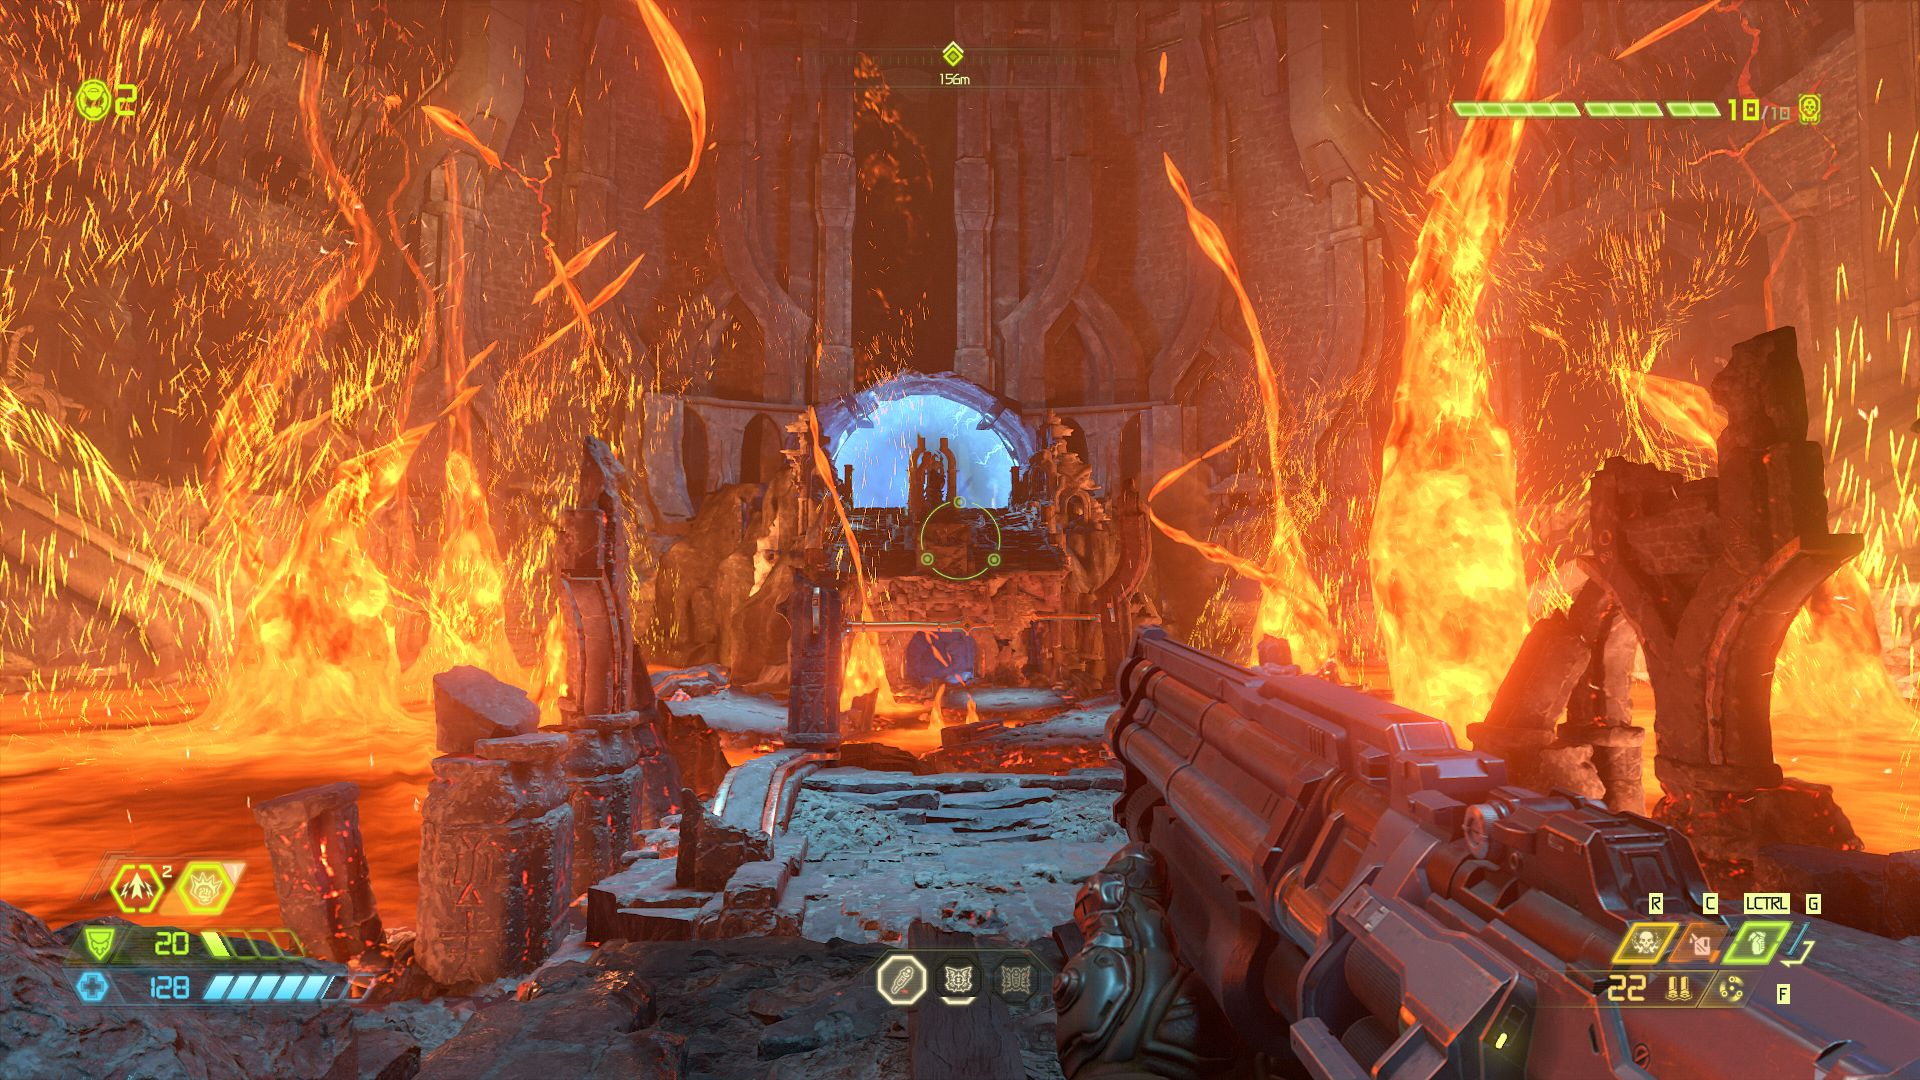
\includegraphics[width=0.5\textwidth]{DoomEternal}
    \caption{Кадр из игры Doom Eternal}%
    \label{fig:doomEternal}
\end{wrapfigure}
\begin{itemize}
    \item средняя частота кадров сцены --- 60 кадров /сек.;
    \item максимальная визуальная привлекательность;
    \item адаптивность под задачи художников.
\end{itemize}
\end{frame}

\section{Постановка задачи}
\begin{frame}
\frametitle{Цели и задачи исследования}
\textbf{Объектом исследования} является огонь в трехмерной графике как один из
элементов трехмерной сцены.

\textbf{Предметом исследования} является динамическая симуляция объемного огня в
режиме реального времени.

\textbf{Цель исследования} --- разработка системы динамической симуляции
трехмерного огня.

\textbf{Задачи исследования:}
\begin{enumerate}
	\item Обзор и анализ научных работ по современным алгоритмам анимации огня и
        трехмерному рендерингу.
	\item Анализ теории динамической симуляции огня.
	\item Реализация системы динамической симуляции.
\end{enumerate}
\end{frame}

\section{Анализ литературных источников}
\begin{frame}
\frametitle{Анализ методов симуляции огня}
В 2011 году Чжао Хуэй и его коллеги представили статью~\cite{survey}, в которой
авторы проанализировали большое количество методов симуляции огня и предложили
свою классификацию методов.

Результаты данного исследования можно увидеть в
таблице~\ref{table:algoAnalsysis}.
\begin{table}[htb]
    \caption{Сравнение производительности различных методов симуляции огня}
    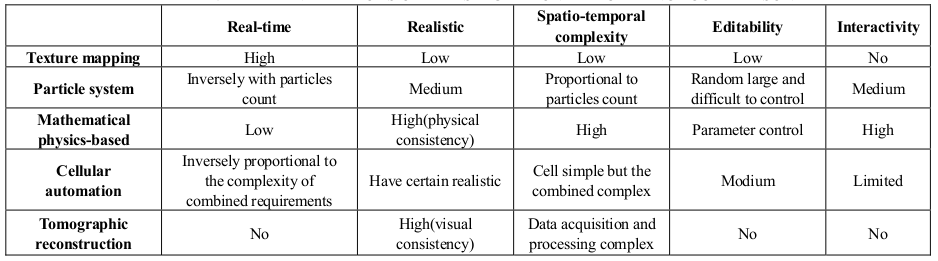
\includegraphics[width=\textwidth]{simulation_methods}%
    \label{table:algoAnalsysis}
\end{table}
\end{frame}

\section{Теория динамической симуляции огня}
\begin{frame}
\frametitle{Структура симуляции}
В общем случае задача симуляции огня может быть разбита на три
непересекающихся подзадачи~\cite{Perry94synthesizingflames}:
\begin{wrapfigure}{r}{0.5\textwidth}
	\centering
    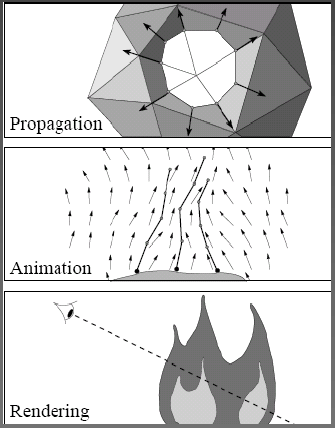
\includegraphics[width=0.27\textwidth]{simStages}
    \caption{Структура симуляции, предложенная в~\cite{realistic_sim}}%
    \label{fig:simStages}
\end{wrapfigure}
\begin{itemize}
	\item моделирование;
	\item анимация;
	\item визуализация.
\end{itemize}
Альтернативная схема была предложена Филиппом Боденом в
работе~\cite{realistic_sim} (рис.~\ref{fig:simStages}).
\end{frame}

\section{Техническое решение}
\begin{frame}
\frametitle{Идея решения}
В процессе анализа предыдущих работ по данной теме были выделены следующие идеи,
которые легли в основу технического решения:
\begin{enumerate}
    \item Визуальная эффектность симуляции важнее реалистичности.
    \item Физико-математические методы позволяют достичь высокой реалистичности
        анимации, однако требуют больших затрат ресурсов.
    \item Использование аналогий при анимации позволит существенно
        уменьшить количество расчетов по сравнению с численными методами.
\end{enumerate}
\end{frame}

\subsection{Компоненты решения}
\begin{frame}
\frametitle{Моделирование}
В качестве модели системы была выбрана система частиц, впервые предложенная в
Уильямом Томасом Ривзом в 1983 году в работе~\cite{reewes1983}.

В качестве основы для симулятора была использована система для генерации частиц
в 2D игре, предложенная в работе~\cite{LearnOGL}. В систему были внесены
следующие оптимизации:
\begin{itemize}
    \item Система полностью адаптирована для работы в 3D пространстве.
    \item Алгоритмы рендеринга были оптимизированы, что позволило увеличить
        число частиц в системе с нескольких сотен до десятков тысяч.
    \item Увеличено количество атрибутов частиц.
\end{itemize}
\end{frame}

\begin{frame}
\frametitle{Структура симуляции}
В качестве структуры симулятора была выбрана схема, предложенная
в работе~\cite{Somasekaran2005UsingPS}. Общая структура симулятора представлена
на рисунке~\ref{fig:simStructure}.
\begin{figure}[htb]
	\centering
	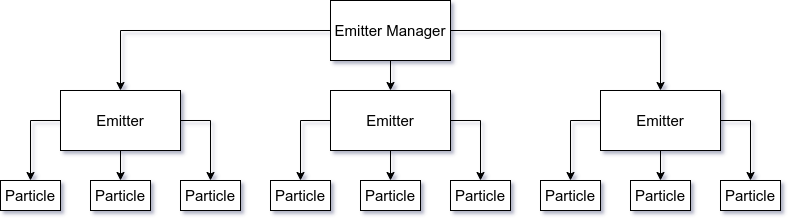
\includegraphics[width=\textwidth]{Structure}
    \caption{Иерархия объектов, использованная в разработанном симуляторе}%
    \label{fig:simStructure}
\end{figure}
\end{frame}

\begin{frame}[t]
\frametitle{Схема обновления частиц}
\begin{wrapfigure}{R}{0.5\textwidth}
	\centering
	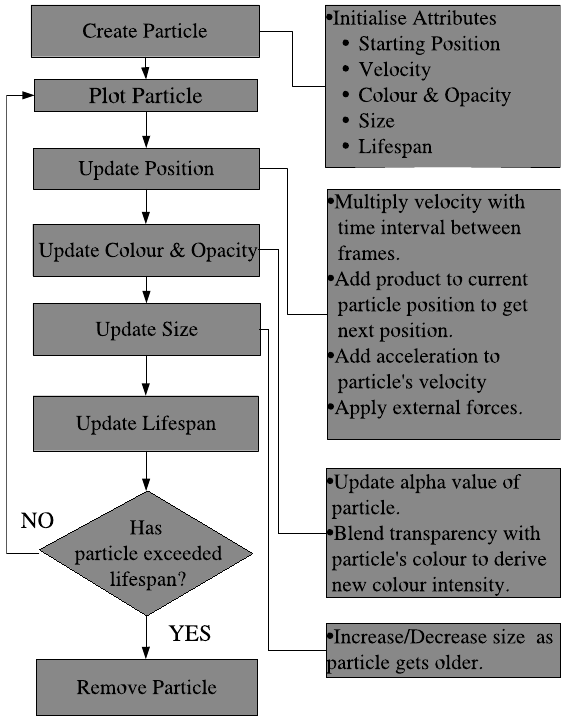
\includegraphics[height=6.2cm]{algorithm}
    \caption{Схема обновления частиц в кадре}%
    \label{fig:algorithm}
\end{wrapfigure}
В качестве основы алгоритма обновления частиц была использована схема,
предложенная Вудхаузом в публикации~\cite{Woodhouse} (рис.~\ref{fig:algorithm}).

На шаге обновления позиции также выполняется генерация точек низкого давления
давления для анимации частиц и расчет траектории частиц.
\end{frame}

\begin{frame}
\frametitle{Промежуточные результаты}
На рисунке~\ref{fig:proto4} представлен промежуточный прототип. В данном
прототипе все частицы движутся равноускоренно и прямолинейно в сторону эмиссии.
\begin{figure}[htb]
	\centering
    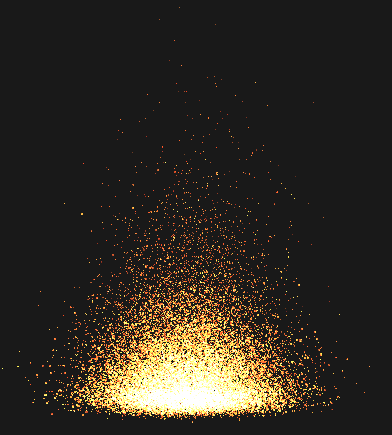
\includegraphics[width=0.35\textwidth]{proto4}
    \caption{''Наивная'' анимация}%
    \label{fig:proto4}
\end{figure}
\end{frame}

\begin{frame}
\frametitle{Анимация частиц}
Для анимации частиц был использован алгоритм, предложенный
в работе~\cite{Somasekaran2005UsingPS}.
\begin{figure}[htb]
	\centering
    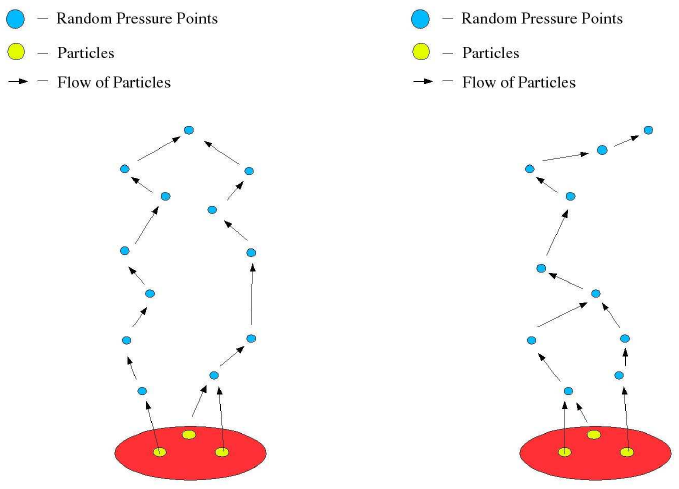
\includegraphics[height=5cm]{animationAlgo}
    \caption{Алгоритм анимации частиц}%
    \label{fig:animationAlgo}
\end{figure}
\end{frame}

\begin{frame}
\frametitle{Реализация анимации}
Реализованная анимация позволила добиться реалистичного движения языка пламени.
\begin{figure}[htb]
	\centering
    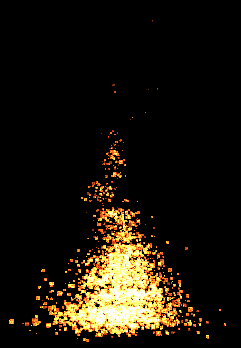
\includegraphics[height=5.5cm]{protoFinal}
    \caption{Реализация анимации частиц}%
    \label{fig:protoFinal}
\end{figure}
\end{frame}

\begin{frame}[t]
\frametitle{Текстурные сплэты}
\begin{wrapfigure}{r}{0.3\textwidth}
	\centering
    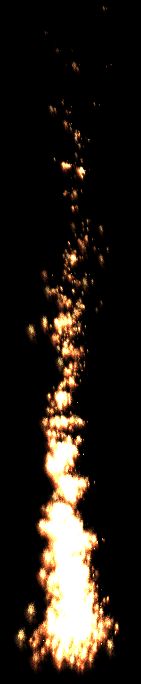
\includegraphics[height=5.5cm]{simSplats}
    \caption{Использование текстурных сплэтов для рендеринга частиц}%
    \label{fig:protoSplats}
\end{wrapfigure}
Для улучшения рендеринга можно использовать текстурные сплэты --- текстуры с
альфа-каналом, которые накладываются друг на друга~\cite{FireSplats}.Для
увеличения стохастичности следует чередовать различные текстуры.

Недостатки метода:
\begin{itemize}
    \item необходимо ориентировать полигоны на зрителя;
    \item нереалистичные результаты при наблюдении сверху.
\end{itemize}
\end{frame}

\subsection{Экспериментальные результаты}
\begin{frame}
\frametitle{Производительность системы}
Одним из важных экспериментов является поиск максимального количества частиц в
системе, при котором сохраняется приемлемая частота кадров
(таблица~\ref{table:amountBench}).
Окружение симуляции использует операционную систему Debian 10 Buster, процессор
Intel Core i5-5200U с частотой 2.7GHz, 8 ГБ оперативной памяти и видеокарту
Intel(R) HD Graphics 5500.
\begin{table}[htb]
\caption{Зависимость частоты кадров от количества частиц в системе}%
\label{table:amountBench}
\centering
\small
\begin{tabular}{| l | l |}
    \hline
    Количество частиц & Средняя частота кадров \\
    \hline
    5000 &  60,00 \\
    \hline
    10000 & 58,46 \\
    \hline
    15000 & 50,62 \\
    \hline
    25000 & 31,94 \\
    \hline
    50000 & 15,85 \\
    \hline
\end{tabular}
\end{table}
\end{frame}

\begin{frame}[t,allowframebreaks]
\frametitle{Список использованных источников}
\sloppy\printbibliography[
    notcategory=AuthorSources,
    heading=none,
    resetnumbers,
]
\end{frame}

% \begin{frame}
% \frametitle{Outline}
% \tableofcontents
% \end{frame}
